\section{Software testing}
\label{sec:related:testing}

Software testing is the process of executing a program or system
with the intent of finding errors \cite{Myers:1979:AST:539883}.
However, testing shows the presence, not the absence of bugs as
Edsger Wybe Dijkstra used to say \cite{Buxton:1970:SET:1102021}.

Testing is achieved by analysing a software to detect the
differences between existing and required conditions (that is,
bugs) and to evaluate the features of this software. As Myers
said \cite{Myers:1979:AST:539883}, testing is used to find
faults, but it is also useful to provide confidence of
reliability, correctness, and absence of particular faults on
software we develop. This does not mean that the software is
completely free of defects. Rather, it must be good enough for
its intended use.  Testing is a verification and validation
(V\&V) process \cite{wallace1989software}. I use to (informally)
explain both terms with the following questions \cite{Boehm1979}:

\begin{itemize}
    \item \textbf{Validation:} are we building the right software?
    \item \textbf{Verification:} are we building the software right?
\end{itemize}

In other words, formal verification is the act of proving or
disproving the correctness of intended algorithms underlying a
system with respect to a certain formal specification or
property, using formal methods of mathematics. Model checking,
runtime verification, theorem proving, static analysis and
simulation are all verification methods.

Validation is testing as the act of revealing bugs. That is what
most people think testing is, and also the meaning we give to the
word "testing" in the sequel of this thesis. Testing involves a
(software) \textit{system under test} (SUT). The prevailing
intuition of testing is reflected in its operational
characterization as an activity in which a \textit{tester} first
generates and sends stimuli, i.e. \textit{test input} data, to a
system under test in order to observe phenomena (mainly
behaviors). Such phenomena can be represented by the existence of
\textit{test outputs} for instance. We then have to decide on a
suitable \textit{verdict}, which expresses the assessment made.
The two most well-known verdicts are $Pass$ and $Fail$.
We call \textit{test case} (TC), a structure that is compound of
\textit{test data}, i.e.  inputs which have been devised to test
the system, an expected behavior, and an expected output. A set
of test cases is called a \textit{test suite} (TS).

In the following section, we introduce the software testing
realm. We focus on Model-based Testing, presented in Section
\ref{sec:related:testing:mbt} along with some definitions used
in the rest of this thesis.

\subsection{Types of testing}

\begin{figure}[ht]
    \begin{center}
    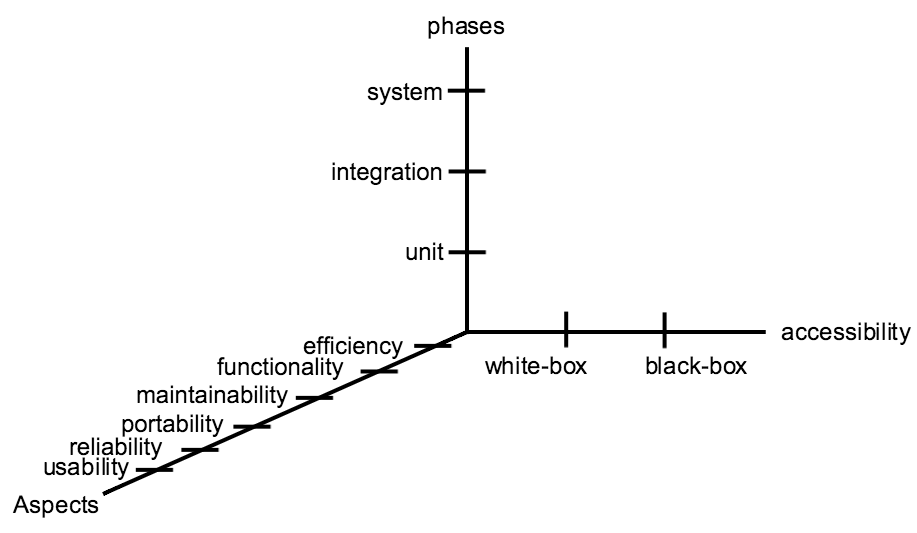
\includegraphics[width=1.0\linewidth]{figures/sorts-of-testing.png}
    \end{center}

    \caption{Sorts of testing. We can sort testing techniques by
    aspect (characteristics of quality), by phase (related to the
    target of the test), and by accessibility (related to the
    information available to construct the test cases).}
\end{figure}

Nowadays, software testing, if not always applied, is well-known
in the Industry. It is considered a good practice and many
techniques and tools have been developed over the last 10 years.
Most of them are different in nature and have different purposes.
There are a lot of new terms that all end with "Testing" such as:
Unit Testing, Integration Testing, Functional Testing, System
Testing, Stress Testing, Performance Testing, Usability Testing,
Acceptance Testing, Regression Testing, Beta Testing, and so on.

ISO 9126 \cite{iso9126}, replaced by ISO/IEC 25010:2011
\cite{10951538}, provides six characteristics of quality that can
be used to sort these testing techniques into six testing types:

\begin{itemize}
\item Efficiency testing;
\item Functionality testing;
\item Maintainability testing;
\item Portability testing;
\item Reliability testing;
\item Usability testing.
\end{itemize}

However, this classification can not be generally accepted as
single or complete. In \cite{4425813}, authors suggested to
classify the different techniques based on the target of the
test (sometimes we refer to this classification as level of
detail):

\begin{itemize}
\item \textbf{Unit Testing:} units (e.g., functions, methods,
modules) of the system are tested in isolation. Typically this
testing type implies access to the source code being tested;

\item \textbf{Integration Testing:} interactions between software
components are tested. This testing type is a continuous task,
hence the \textit{continous integration} (CI) practice;

\item \textbf{System Testing:} the whole system is taken into
consideration. This testing type is appropriate for validating
not-only-functional requirements, such as security, performance
(speed), accuracy, and reliability (fault tolerence).
\end{itemize}

These requirements are sometimes seen as \textit{objectives} of
testing, leading to even more different testing types as listed
before. There are also different approaches (or perspectives) to
perform testing, depending on the information available to
construct the test cases, i.e. accessibility:

\begin{itemize}
    \item \textbf{White-box:} a method that tests the internal
        structure of a SUT. It is usually done at the unit level;

    \item \textbf{Black-box:} a method that tests the functionalities
        of a SUT without knowing its internal structure. The behavior
        of the \textit{implementation under test} (IUT) is only
        visible through a restricted interface called \textit{Points
        of Control and Observation} (PCOs). Such a technique is also
        known as functional testing;

    \item \textbf{Grey-box:} the combination of white-box testing and
        black-box testing. One has access to the relevant internal
        parts of a SUT.
\end{itemize}

\subsubsection{Test selection}

Because testing cannot guarantee the absence of faults, a
challenge is to select subset of test cases from all possible
test cases with a high chance of detecting most faults. A lot of
research on \textit{test selection} (or strategies) has been
done, and there are numerous existing methods for both black-box
and white-box approaches.

\paragraph{Black-box strategies} Combinatorial Testing (also
known as Pairwise) \cite{Tai98atest} is based on the observation
that most faults are caused by interactions of at most two
factors. Here we test all the possible discrete combinations of
the parameters involved.  Because we cannot test all the possible
input domain values for practical reasons, Equivalence
Partitioning \cite{Huang13} is a technique that divides the test
input data into a range of values, and selects one input value
from each range. Similarly, Boundary Value Analysis
\cite{Ramachandran:2003:TSC:942796.943301} is used to find the
etechniquesrrors at boundaries of input domain rather than finding those
errors in the center of input. We can also mention Functional
Coverage (also known as Inductive Testing)
\cite{Walkinshaw:2010:IFC:1928028.1928038} where a test set is
good enough when it achieves a given level of coverage.

\paragraph{White-box strategies} Fuzz Testing also known as
Random Testing
\cite{Duran:1981:RRT:800078.802530,Godefroid08automatedwhitebox}
is a method that applies random mutations to well-formed inputs
of a program, and test the resulting values. Such a technique can
also be applied using a black-box approach though, e.g.,
\cite{5387827}.  Statistical Testing
\cite{Walton:1995:STS:210453.210458} is a technique where test
data is generated by sampling from a probability distribution
chosen so that each element of the software's structure is
exercised with a high probability. We can also mention all
techniques related to the code structure, such as Statement
Testing, Path Testing, Branch Testing, Condition Testing,
Multiple Condition (MC) Testing, and Loop Testing.  Another
technique acts on the source code by mutating it, i.e.  seeding
the implementation with a fault by applying a mutation operator,
and then determining whether testing identifies this fault. This
is known as Mutation Testing \cite{1702444}.

While the Industry created many different testing tools (often
originating from Academia), they mostly perform testing by hand.
Researchers in software testing have worked for decades on
automatic test generation. Automatic testing is, for instance,
one way to automate white-box approaches, but there are many
other techniques. On the contrary, Model-based Testing (MbT) is
one research area that tries to automate black-box approaches.
In this thesis, we are interested in making production systems
more reliable by means of Model-based Testing.

\subsection{Model-based Testing}
\label{sec:related:testing:mbt}

\begin{figure}[ht]
    \begin{center}
    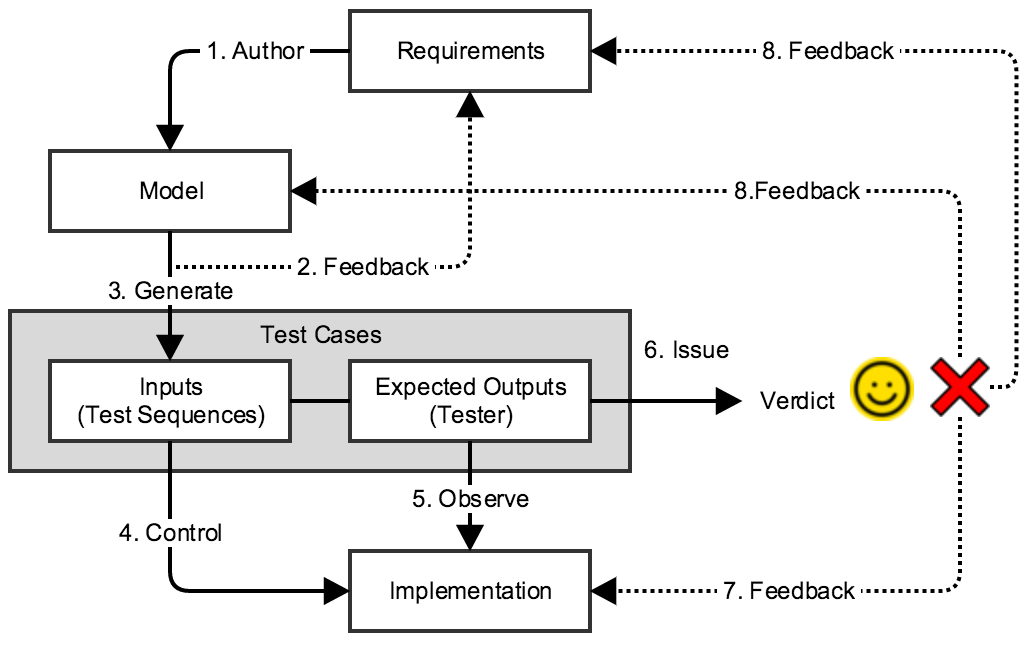
\includegraphics[width=1.0\linewidth]{figures/mbt.png}
    \end{center}

    \caption{A simplified diagram showing how MBT works. This is
    a three-step process.}
    \label{fig:mbt}
\end{figure}
\TODO{Figure: test oracle => tester}

\textit{Model-based Testing} (MbT) is application of Model-based
design for designing and optionally also executing artifacts to
perform software testing \cite{Jorgensen:1995:STC:526521}.
Models can be used to represent the desired behavior of an SUT,
or to represent testing strategies and a test environement.
Model-based Testing can be summarized as a three-step process,
which is extended in Figure \ref{fig:mbt}:

\begin{enumerate}
\item Formally modeling the requirements (specification);

\item Generating test cases from the model;

\item Running these test cases against an actual SUT and
evaluating the results.
\end{enumerate}

\subsubsection{What is a model?}
\label{sec:related:testing:model}

Generally speaking, a model is a representation of a thing that
allows for investigation of its properties, and most of the time,
a model hides the complexity of the item it represents. In the
software engineering field, models help describe software systems
in order to: (i) ease the process of studying them, (ii) leverage
them to build tools or generate documentation, (iii) reveal
defects (validation or verification).

Such models usually describe the behaviors of the software being
modeled, and can also be known as specifications, helping
understand and predict its behavior. There are numero models for
modeling software systems, and each describes different aspects
of software behavior. For example, control flow, data flow, and
program dependency graphs express how the implementation behaves
by representing its source code structure. It is worth mentioning
that a model does not have to completely describe it to be
effective.

We can classify models that can be employed for testing into two
categories (these lists are not exhaustive):

\begin{itemize}
    \item \textbf{Behavior/Control oriented:} Finite Automata (like
        Finite State Machines, Symbolic Transition Systems, and Labelled
        Transition Systems) are well-known in software testing. They are
        very generic and flexible, and are a good fit when it comes to
        model software systems. For real-time and/or safety-critical
        systems, we often rely on Synchronous Languages such as Lustre
        \cite{lustre:ieee} and SCADE
        \cite{LeSergent:2011:SCF:2188575.2188578}. We can also mention
        Petri Nets, Finite State Machines, and timed automata
        \cite{Alur94atheory};

    \item \textbf{Data oriented (pre/post):} often using annotation
        languages originating from the \textit{Design-By-Contract}
        paradigm \cite{Meyer:1992:ADC:618974.619797}. These languages
        make it possible to express formal properties (invariants,
        pre/post-conditions) that directly annotate program entities
        (such as classes, methods, attributes) in the source code. Many
        annotation languages exist, such as the Java Modeling Language
        \cite{jml}, Spec\# \cite{117852}, the Object Constraint Language
        \cite{Warmer:1998:OCL:291202}, the B-Method
        \cite{Lano:1996:BLM:525749}, and Praspel
\cite{Enderlin:2011:PSL:2075545.2075551}.
\end{itemize}

In \cite{Sommerville:1997:REG:549198}, Sommerville and Sawyer
give some guidelines for choosing a model for software
requirements. The choice of a model depends on many factors, such
as aspects of the system under test or the testing goal.  Below
we introduce a few definitions of formal models that we use in
this thesis. We mainly work with behavior-oriented models that
are finite automata since they are particularly suitable for
modeling both web applications and production systems behaviors.

\subsubsection{Model definitions}

\paragraph{Labelled Transition Systems}
\label{sec:definitions:lts}

A \textit{Labelled Transition System} is a model compound of
states with transitions, labelled with actions, between them.
The states model the system states and the labelled transitions
model the actions that a system can perform.

We give the definition of the LTS model below, but we refer to
\cite{ltsTretmans} for a more detailed description.

\begin{definition}[Labelled Transition System]
    A labelled transition system is a 4-tuple $<Q,L,T,q_0>$ where:

    \begin{itemize}
    \item $Q$ is a countable, non-empty set of state;

    \item $L$ is a countable set of labels;

    \item $T \subseteq Q \times (L \cup \{\tau\}) \times Q$, with
    $\tau \not\in L$, is the transition relation;

    \item $q_0 \in Q$ is the initial state.

    \end{itemize}

    We write $q \xrightarrow[]{t} q'$ if there is a transition
    labelled $t$ from state $q$ to state $q'$ , i.e., $(q, t, q')
    \in T$.

	\label{def:lts}
\end{definition}


\paragraph{Symbolic Transition Systems}
\label{sec:definitions:sts}

The \textit{Symbolic Transition System} (STS) is known as a very
general and powerful model for describing several aspects of
event-based systems. The use of symbolic variables
helps describe infinite state machines in a finite manner. This
potentially infinite behaviour is represented by the semantics of
a STS, given in terms of \textit{Labelled Transition System}
(LTS). STS operations and transformations are often given with
inference rules.

We give some definitions related to the STS model below, but we
refer to \cite{FTW05} for a more detailed description.

\begin{definition}[Variable assignment]
We assume that there exist a domain of values denoted by $D$ and
a variable set $X$ taking values in $D$. The assignment of
variables in $Y \subseteq X$ to elements of $D$ is denoted by
$\alpha: Y \rightarrow D$. $\alpha(x)$ denotes the assignment of
the variable $x$ to a value in $D$.

We denote by $D_Y$ the assignment set over $Y$. We also denote by
$id_Y$ the identity assignment over $Y$. Finally, $v_\emptyset$
is the empty assignment.
\end{definition}

\begin{definition}[Symbolic Transition System]
	A Symbolic Transition System (STS) consists of locations and
    transitions between locations. It is defined as a tuple $<
    L,l0,V,V0,I,\Lambda,$ $\rightarrow>$, where:

	\begin{itemize}
        \item STSs do not have \textbf{states but locations}
        (a.k.a. symbolic states), and $L$ is the finite location
        set, with $l0$ being the initial one;

        \item $V$ is the finite set of internal variables, while
        $I$ is the finite set of parameters. The internal
        variables are initialised with the condition $V0$ on
        $V$;

        \item $\Lambda$ is the finite set of symbolic actions
        $a(p)$ ($a$ being a symbol), with $p=(p_1,\dots ,p_k)$ a
        finite set of parameters in $I^{k} (k \in \mathbb{N})$;

        \item $\rightarrow$ is the finite set of symbolic
            transitions. A symbolic transition $t =
            (l_i,l_j,a(p),G,\\A)$, from the location $l_i \in L$
            to $l_j \in L$, also denoted by $l_i
            \xrightarrow{a(p),G,A} l_j$, is labelled by:

		\begin{itemize}
            \item an action $a(p) \in \Lambda$;

            \item a guard $G$ over $(p \cup V)$, which
            restricts the firing of the transition. Throughout
            this thesis, we consider guards written as
            conjunctions of equalities: $\displaystyle
            \bigwedge_{x \in I \cup V} (x == val)$;

            \item an assignment $A$ which defines the evolution
            of the proper variables, $A_x$ being the function in
            $A$ defining the evolution of the variable $x \in V$.
		\end{itemize}
	\end{itemize}

	\label{def:sts}
\end{definition}

We also denote by $Proj_{x}(G)$ the projection of the guard $G$ over
the variable $x \in I \cup V$, which extracts the equality
$(x==val)$ from $G$. For example, given the guard $G_1 = [nsys==1
\wedge nsec==8 \wedge point==1 \wedge pid==1]$, $Proj_{nsys}(G_1)
= (nsys==1)$.

For readability purpose, if $A$ is the identity function $id_V$,
we denote a transition by $l_i \xrightarrow{a(p),G} l_j$. We
also use the generalised transition relation $\Rightarrow$ to
represent STS paths: $l \xRightarrow{(a_1,G_1,A_1)\dots
(a_n,G_n,A_n)} l' =_{def} \exists l0\dots l_n, l=l0
\xrightarrow{a_1,G_1,A_1} l_1\dots
l_{n-1}\xrightarrow{a_n,G_n,A_n}l_n=l'$.

\paragraph{Labelled Transition System semantics}
\label{sec:definitions:lts-semantics}

A STS is associated with a Labelled Transition System (LTS) to
formulate its semantics. Intuitively, a LTS semantics corresponds
to a valued state machine, without symbolic variables, which is
often infinite: the LTS states are labelled by internal variable
assignments while transitions are labelled by actions combined
with parameter assignments.

\begin{definition}[Labelled Transition System semantics]
    The semantics of a STS $\EuScript{S}=<L,l0,$ $V,$ $V0,$
    $I,\Lambda,\rightarrow>$ is the LTS
    $||\EuScript{S}||=<Q,q_0,\sum,\rightarrow>$ where:

	\begin{itemize}

		\item $Q=L \times D_V$ is the set of states;

        \item $q_0=(l0,V0)$ is the initial state;

		\item $\sum=\{(a(p),\alpha)  \mid  a(p)\in\Lambda, \alpha \in
		D_p\}$ is the set of valued events;

        \item $\rightarrow$ is the transition relation $Q \times
        \Sigma \times Q$ deduced by the following rule:\\
	\end{itemize}
	\begin{center}
    {\Large
    $\frac{l_1 \xrightarrow{a(p),G,A}l_2,\alpha \in D_p, v \in D_V, v'
        \in D_V, v \cup \alpha \models G, v'=A(v \cup \alpha))}{(l_1,v)
            \xrightarrow{a(p),\alpha} (l_2,v') }$
    }
	\end{center}

	\label{def:semantics}
\end{definition}

This rule can be read as follows: for a STS transition $l_1
\xrightarrow{a(p),G,A}l_2$, we obtain a LTS transition $(l_1,v)$
$\xrightarrow{a(p),\alpha} (l_2,v')$ with $v$ a variable
assignment over the internal variable set, if there exists an
assignment $\alpha$ such that the guard $G$ evaluates to true
with $v \cup \alpha$. Once the transition is executed, the
internal variables are assigned with $v'$ derived from the
assignment $A(v \cup \alpha)$.

In addition, runs and traces, which represent executions and
event sequences, can also be derived from LTS semantics:

\begin{definition}[Runs and traces]
    Given a STS $\EuScript{S}=$ $<L,l0,V,V0,I,\Lambda,
	\rightarrow>$, interpreted by its LTS semantics
	$||\EuScript{S}||=<Q,q_0,\sum,\rightarrow>$, a run $q_0
	\alpha_0 \dots \alpha_{n-1} q_n$ is an alternate sequence of states
    and valued actions. $Run(\EuScript{S})=Run(||\EuScript{S}||)$ is
	the set of runs found in $||\EuScript{S}||$.

    It follows that a trace of a run $r$ is defined as the
    projection $proj_{\sum}(r)$ on the actions.

	\label{def:runs-and-traces}
\end{definition}

\paragraph{Input/Output Symbolic Transition Systems}
\label{sec:definitions:iosts}

An Input/Output Symbolic Transition System (IOSTS) is a STS where
the action set is divided into two subsets: one containing the
inputs, beginning by $?$, to express actions expected by the
system, and another containing outputs, beginning by $!$, to
express actions produced by the system.

\begin{definition}[Input/Output Symbolic Transition System]
An Input/Output Symbolic Transition System (IOSTS) $\EuScript{S}$
is a tuple $< L,l0,V,V0,I,\Lambda,\rightarrow>$, where:

\begin{itemize}
\item $L$ is the finite set of locations, $l0$ the initial
location;

\item $V$ is the finite set of internal variables, $I$ is the
finite set of parameters. The internal variables are initialised
with the assignment $V0$ on $V$, which is assumed to be unique;

\item $\Lambda$ is a finite set of symbolic actions $a(p)$, with
$p = (p_1,\dots,p_k)$ a finite list of parameters in $I^k(k \in
\mathbb{N})$. $p$ is assumed unique. $\Lambda= \Lambda^I  \cup
\Lambda^O \cup \{!\delta \}$: $\Lambda^I$ represents the set of
input actions, $\Lambda^O$ the set of output actions, and
$\delta$ the quiescence;

\item $\rightarrow$ is the finite transition set. A transition
$(l_i,l_j,a(p),G,A)$, from the location $l_i \in L$ to $l_j \in
L$, denoted by $l_i \xrightarrow{a(p),G,A} l_j$ is labelled by: an
action $a(p) \in \Lambda$, a guard  $G$ over $(p \cup V \cup T(p
\cup V))$ that restricts the firing of the transition. $T(p \cup
V)$ is a set of functions that return boolean values only (a.k.a.
predicates) over $p \cup V$, an assignment function $A$ that
updates internal variables. $A$ is on of the form $(x:=A_x)_{x\in
V}$, where $A_x$ is an expression over $V \cup p \cup T(p \cup
V)$.
\end{itemize}
\end{definition}

\subsubsection{Common terms in MbT}

In this section, we introduce a few common terms defining what
Model-based Testing is, and how it works in general.

Executing a test case on a system yields a set of observations.
Every observation represents a part of the \textit{implementation
model} of the system. The set of all observations made with all
possible test cases represents the complete implementation model
of the system.

\paragraph{Testing hypothesis} For every system there is a
corresponding observational equivalent implementation model:
$\forall \text{ } iut \in IMPS, \exists \text{ } I_{iut} \in
MODS$, where $iut$ is a concrete implementation under test,
$IMPS$ is the universe of implementations, $I_{iut}$ is a model
of $iut$, and $MODS$ is the universe of the models of all IUT.

\paragraph{Implementation relation} To define conformance between
an implementation under test $imp$ and a specification $spec$, we
use the notion of an \textit{implementation relation}: $imp
\subseteq MODS \times SPECS$, with $SPECS$ the set of
specifications. We can find different implementation relations,
e.g., \cite{Bri88,phalippou94}.

\paragraph{Conformance} An implementation $iut$ conforms to a
specification $spec$ if the existing model $I_{iut}$ of $iut$ is
\textit{imp-related} to $spec$. There are many conformance
relations in the literature, which we can organize in three
categories:

\begin{itemize}
    \item \textbf{Equivalence relations:} Isomorphism,
        Bisimulation
        \cite{Abdulla06,Fernandez89animplementation}, Trace
        Equivalence, Testing Equivalence \cite{Abramsky1987225},
        Refusal Equivalence \cite{Phillips86};

    \item \textbf{Preorder relations:} Observation Preorder,
        Trace Preorder \cite{DNH84}, Testing Preorder
        \cite{Beohar2015}, Refusal Preorder;

    \item \textbf{Input-Output relations:} Input-Output Testing,
        Input-Output Refusal, ioconf
        \cite{tretmans1996conformance}, ioco \cite{Tre96}.
\end{itemize}

\paragraph{Conformance testing} Conformance Testing assesses
conformance to an unknown implementation under test $iut$ to its
specification $spec$ by means of test experiments. Experiments
consist of stimulating $iut$ in certain ways and observing its
reactions. This process is called \textit{test execution}.

\paragraph{Test execution} The successful execution of a test
case $TC$ can be written as follows: $I_{iut} \text{ }
\mathbf{passes} \text{ } TC$. We can easily extend it to a test
suite $TS$: $I_{iut} \text{ } \mathbf{passes} \text{ } TS
\Leftrightarrow \forall \text{ } TC \in TS : I_{iut} \text{ }
\mathbf{passes} \text{ } TC$. On the contrary, $I_{iut} \text{ }
\mathbf{fails} \text{ } TC \Leftrightarrow I_{iut} \text{ } \neg
\mathbf{passes} \text{ } TC$.

This leads to three properties on the test suite $TS$:

\begin{itemize}
\item \textbf{Soundness:} $\forall \text{ } iut \in IMPS, iut$
conforms to $spec \implies iut \text{ } \mathbf{passes} \text{ }
TS$;

\item \textbf{Exhaustiveness:} $\forall \text{ } iut \in IMPS,
iut \text{ } \mathbf{passes} \text{ } TS \implies iut$ conforms
to $spec$;

\item \textbf{Completeness:} $\forall \text{ } iut \in IMPS, iut$
conforms to $spec \Leftrightarrow iut \text{ } \mathbf{passes}
\text{ } TS$.
\end{itemize}

We rely on a \textit{test architecture}, i.e. an abstract
description of the \textit{environment} in which an
implementation under test $iut$ is embedded, and where it
communicates with a \textit{tester}.

\paragraph{Tester and verdicts} A tester executes the test cases.
To be able to decide about the success of each, a
\textit{verdict} (most of the time, $pass$ or $fail$) is attached
to each state of each test case.


\subsection{(Active and) passive testing}

In this section, we introduce two different approaches based on
how we apply the test cases to the system under test:

\begin{itemize}
    \item \textbf{Active testing}, which is the classical process
        in which a tester examines the functionality of a unit
        under test before that unit is being deployed, i.e.
        during its development;

    \item \textbf{Passive testing}, which takes place after the
        deployment of that unit, and requires, for instance, the
        presence of a \textit{monitor}. Passive testing is also
        useful when one wants to test a system during a long
        period of time.
\end{itemize}

While active testing can take place as black- or white-box
testing, passive testing is often a special form of black-box
testing. Active testing works by stimulating the system under
test, i.e. observing outputs of an implementation for predefined
inputs. Most of the classical testing techniques and tools found
in the Industry perform active testing, e.g., \textit{xUnit}
frameworks
\footnote{\url{http://www.martinfowler.com/bliki/Xunit.html}}.

Passive testing rather examines the input/output behavior of an
implementation without predefining the input. One advantage of
passive testing is that it does not disturb the system, and it
can be applied on large (distributed) systems. While most of the
works on passive testing are related to networks, protocols, and
web services, such a technique can be particularly suitable for
production systems.

Several works, dealing with passive testing of protocols or
components, have been proposed over the last decade. For all of
these, the tester is made up of a module, located in the
implementation environment, which collects trace sets. These
works can be grouped in three different categories.

\subsubsection{Invariant satisfiability}

Invariants represent properties that are always true. They are
constructed by hand from a specification, and later checked on
the collected traces. Similarly to runtime verification
\cite{Leucker2009293}, this approach allows to test complex
properties on an implementation. It gave birth to several works
in the literature. For instance, the passive testing method,
presented in \cite{CMdO09}, aims to test the satisfiability of
invariants on Mobile ad hoc network (MANET) routing protocols.
Different steps are required: definition of invariants from the
specification, extraction of execution traces with sniffers,
verification of the invariants on the trace set. Other works
focus on component-based system testing: in this case, passive
methods are usually used to check conformance or security. For
instance, the \textit{TIPS} tool \cite{5552735} performs an
automated analysis of the captured trace sets to determine if a
given set of timed extended invariants are satisfied. As in
\cite{CMdO09}, invariants are constructed from the specification
and traces are collected with network sniffers. Cavalli et al.
propose an approach for testing the security of web service
compositions in \cite{cavalli2009passive}. Security rules are
here modeled with the Nomad language \cite{cuppens2005nomad},
which expresses authorizations or prohibitions by means of
deontic and temporal logics. Preliminary, a rule set is manually
constructed from a specification. Traces of the implementation
are extracted with modules that are placed at each workflow
engine layer that executes web services. Then, the method checks,
with the collected traces, that the implementation does not
contradict security rules. Andrés et al. presented a methodology
to perform passive testing of timed systems in
\cite{andres2012formal}. The paper gives two algorithms to decide
the correctness of proposed invariants with respect to a given
specification and algorithms to check the correctness of a log,
recorded from the implementation under test, with respect to an
invariant.

\subsubsection{Forward checking}

Implementation reactions are given on the fly to an algorithm
that detects incorrect behaviours by covering the specification
transitions with these reactions. Lee et al. proposed a passive
testing method dedicated to wired protocols \cite{1621118}.
Protocols are modeled with \textit{Event-driven Extended Finite
State Machines} (EEFSM), compound of variables.  Several
algorithms on the EEFSM model and their applications to the OSPF
protocol and TCP state machines are presented. Algorithms check
whether partial traces, composed of actions and parameters, meet
a given symbolic specification on the fly. The analysis of the
symbolic specification is performed by means of configuration. A
configuration represents a tuple gathering the current state
label, and a set of assignments and guards modeling the variable
state.

\subsubsection{Backward checking}

Alcalde et al. proposed an approach that processes a partial
trace backward to narrow down the possible specifications in
\cite{alcalde2004network}. The algorithm performs two steps. It
first follows a given trace backward, from the current
configuration to a set of starting ones, according to the
specification. With this step, the algorithm finds the possible
starting configurations of the trace, which lead to the current
configuration. Then, it analyses the past of this set of starting
configurations, also in a backward manner, seeking for
configurations in which the variables are determined.  When such
configurations are reached, a decision is taken on the validity
of the studied paths (traces are completed). Such an approach is
usually applied as a complement to forward checking to detect
more errors.

\subsubsection{Why passive testing?}

It is worth mentioning that passive testing has also been
successfully applied for fault management \cite{965909}, fault
detection \cite{Ural:2007:IAP:1270230.1270259}, and security
purpose \cite{4698175}. To summarize, while passive testing is
less powerful than active testing, because the latter allows a
closer control of the implementation under test, passive testing
still presents interesting advantages:

\begin{itemize}
    \item Passive testing is less costly than active testing in
        general since it does not have to control the
        implementation under test;

    \item Passive testing can be applied to large systems where
        active testing is not even feasible, such as systems with
        many different components, e.g., software oriented
        architectures, distributed systems, but also production
        systems.
\end{itemize}
